\scanpage{66}
% archive foliation: 65

\uline{Th} Sur la cat. $\mathcal E_\infty$ des espaces loc. cpts séparés et \deleted{\unsure{cônes}} ``loc. côniques partout'' (y compris à l'$\infty$), on peut trouver deux fonctions numériques \inserted{$\chi_!,\chi$} (à valeurs $\in\mathbb Z$) satisfaisant les conditions (où tous les espaces écrits sont supposés $\in\mathcal E_\infty$)

\textcircled{a} $\chi_!(X)=\chi(X)$ si $X$ cpt

\textcircled{b} $Y$ fermé dans $X$ $\Longrightarrow\quad\chi_!(X)=\chi_!(Y)+\chi_!(\unsure{Y|X}-Y)$

\textcircled{c} $X',X''$ fermés dans $X$ $\Longrightarrow\quad\chi(X)=\chi(X')+\chi(X'')-\chi(X'\cap X'')$

\textcircled{d}
\[
\left\{\begin{aligned}
X\sim X'&\Longrightarrow\chi(X)=\chi(X')\\
X\simeq X'&\longrightarrow\chi_!(X)=\chi_!(X')
\end{aligned}\right.
\]

\textcircled{e} $\chi(\mathrm{pt})=1$

\textcircled{f}
\[
\begin{aligned}
\chi_!(X\times Y)&=\chi_!(X)\chi_!(Y)\\
\chi_{\deleted{\unsure{!}}}(X\times Y)&=\chi(X)\chi(Y)
\end{aligned}
\]

\textcircled{g} Si $f:X\longrightarrow Y$ fibration loc triviale de fibre $F$,
\[
\left\{\begin{aligned}
\chi_!(X)&=\chi_!(Y)\chi_!(F)\\
\chi(X)&=\chi(Y)\chi(F)
\end{aligned}\right.
\]
tout au moins si $Y$ est un polyèdre relatif (diff. de deux polyèdres, l'un plongé dans l'autre linéairement...)
\margin{j'ignore si c'est vrai sans telle restriction}
\figure{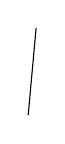
\begin{tikzpicture}\draw (0.1,1.1)--(0,0);\end{tikzpicture}}

Si \deleted{\unsure{le}} $X\in\mathcal E_\infty$ de sorte que $\widehat X\in\mathcal E_\infty$, on a

\textcircled{h}
\[
\left\{\begin{aligned}
\chi_!(X)&=\chi(\widehat X)-1\\
\chi(X)-\chi_!(X)&=\chi(S)\qquad\text{où }S\text{ est le ``}\unsure{\text{frontière}|\text{frontier}}\text{ à l'infini'' de }X.
\end{aligned}\right.
\]

Enfin, \unsure{les restrictions|la restriction} de \deleted{$\unsure{\chi|\mathcal E}$} $\chi$ et $\chi_!$ aux polyèdres relatifs sont uniquement déterminées par les propriétés \textcircled{a} à \textcircled{e}, et on a \deleted{\unsure{le}}, si $X$ muni d'une filtration cellulaire
\[
\chi_!(X)=\sum(-1)^i\unsure{\widehat f_i|f_i}\qquad\text{(formule d'Euler)}
\]
\margin{j'ignore si $\chi$ et $\chi_!$ sont caractérisés par a) à e) sur tout $\mathcal E_\infty$}
\figure{\begin{tikzpicture}\draw (0,1.8) .. controls (-0.1,1.2) and (0.1,0.6) .. (0.25,0);\end{tikzpicture}}

